\newpage

\chapter{Методики вимірювань та теоретичні основи експериментів}

\section{Схема експерименту для дослідження самовпливу}\label{sec:L1}

\begin{figure}
\centering
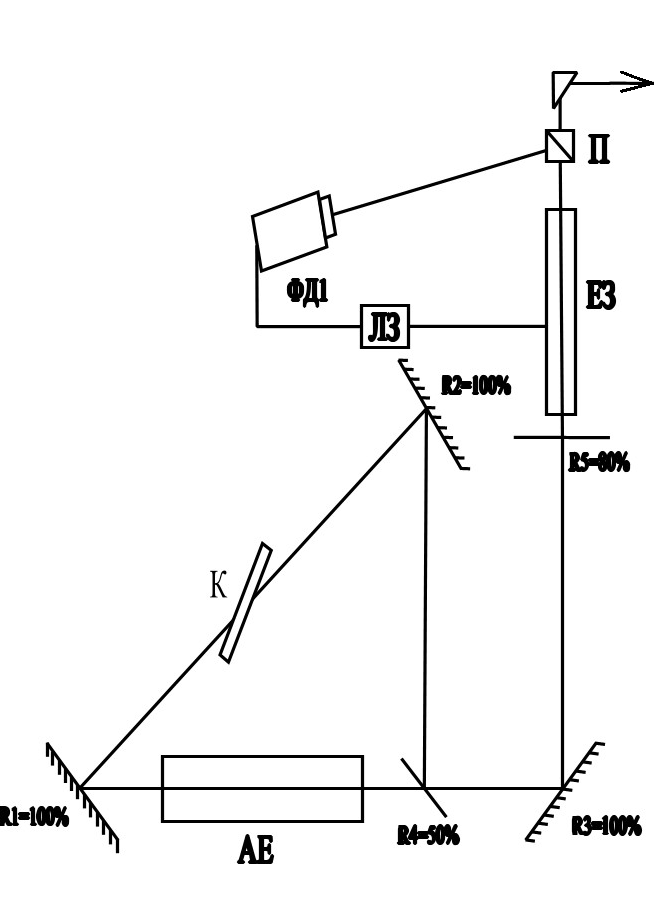
\includegraphics[height=10cm]{las1}
\caption{Оптична схема лазера $Nd^{3+}:\text{АІГ}$ (Л1), що працює в режимі
пасивної синхронізації мод. АЕ -- активний елемент, ФД1 -- фотодіод
виділення одиночного імпульсу, ЕЗ -- електронний затвор, ЛЗ -- лінія
затримки, К -- кювета з барвником. П -- призма Глана, R1-R5 -- дзеркала
(в \% вказані коєфіцієнти відбиття на $\lambda$ = 1064 нм)}\label{fig:las1}
\end{figure}

Оптичну схему лазера Л1 наведено на рис. \ref{fig:las1}.
Резонатор задаючого генератора являє собою інтерферометр Сан'яка з антирезонансним
відбивачем, який складається з подільної пластини (з коефіцієнтом відбиття R4=50\%),
трьох дзеркал (R1=R2=R3=100\%) та вихідного напівпрозорого
дзеркала (R5=80\%). Квантрон з активним елементом розташовується в інтерферометрі Сан'яка,
в оптичному центрі якого знаходиться кювета з
розчином барвника 3274У (поглинач, що просвітлюється під дією оптичного
випромінювання) в етанолі для отримання пасивної синхронізації мод в режимі модуляції добротності.

Вертикальна поляризація лазерного випромінювання в тракті задаючого генератора визначається тим, що кювета
з барвником орієнтована під кутом Брюстера до оптичної осі установки.

Лазер генерує квазімонохроматичне випромінювання на основній
довжині хвилі 1.064 мкм та довжині хвилі другої гармоніки (ДГ) 532 нм в
режимі генерування одиночного імпульсу пікосекундної тривалості при
імпульсній накачці з частотою до 10 Гц. Конструктивно лазер складається із
задаючого генератора, блока виділення одиночного імпульсу з цугу та
перетворювача частоти лазерного випромінювання. 



Для дослідження нелінійно-оптичних властивостей було застосовано оптичну
схему, що наведена на Рис. \ref{fig:s1}. Для зміни інтенсивності лазерного випромінювання,
що потрапляє на зразок, було використано оптичний атенюатор А. Він представляє
собою нейтральний фільтр, імплантований металічними іонами з монотонним
градієнтом поглинання уздовж довшої сторони. Атенюатор має розмір 12.5 см,
оптичне пропускання при цьому змінюються від 1 до 50 \%, таким чином вздовж
області, що підпадає під пучок лазера ($\O \approx 0.5 \text{мм}$) поглинання атенюатора
змінюється незначно. При переміщенні атенюатора лазерний пучок не відхиляється
від початкового напряму.
В системі (Рисунок\ref{fig:s1}) застосовано три вимірювальні канали: опорний канал
(детектор 1), який фіксує потужність випромінювання, відведену поділювачем П1
від пучка, і відповідно, відносну потужність, що падає на зразок; канал повного
пропускання (детектор 2), який вимірює потужність хвилі, яка пройшла крізь зразок
і відведена поділювачем П2; та канал приосьового пропускання (детектор 3), що
вимірює осьову частину профілю пучка, що пройшов крізь діафрагму.
Пучок з гаусовим розподілом інтенсивності фокусується лінзою L на зразок,
що розташований на певній відстані за перетяжкою пучка. Гаусовий просторовий
розподіл інтенсивності лазерного пучка контролюється ПЗЗ лінійкою (AMKO LTI
MuLTIray, 1064 пікселі, розмір пікселя 25 мкм). Діапазон інтенсивності
випромінювання визначається відстанню від зразка до лінзи. Знаючи радіус плями
на вході, відстань від зразку до лінзи та її фокусну відстань, можна однозначно
визначити розмір плями на зразку, що необхідно для розрахунку падаючої
інтенсивності.

Випромінювання, що пройшло крізь зразок, розділяється
поділювальною пластинкою. Частина проходить далі, і в далекому полі вимірюється
осьове пропускання, інша ж частина повертається на 900 і заводиться в канал
вимірювання повної інтенсивності, що пройшла крізь зразок. В цьому каналі перед
вимірювальним пристроєм стоїть збиральна лінза. Це зроблене для мінімізації втрат,
пов’язаних із спотворенням пучка, що пройшов через зразок, та можливим
розсіянням.  

При переміщенні атенюатора змінюється інтенсивність падаючого
випромінювання, що дає можливість реєструвати фотоіндуковану зміну оптичного
пропускання в залежності від інтенсивності. З отриманої залежності визначається
ефективний коефіцієнт ДФП $\beta_{eff}$, що пропорційний до уявної частину ефективної
нелінійної сприйнятливості третього порядку $Im(\chi^{(3)})$.
За рахунок наявності дійсної частини нелінійної кубічної діелектричної
сприйнятливості відбувається зміна ширини та форми профілю лазерного променя.
При проходженні світла крізь НЛО середовище відбувається зміна показника
заломлення в залежності від інтенсивності світла. В найпростішому випадку це
лінійна залежність (керрівська нелінійність).
Одним із способів аналізу фотоіндукованих рефрактивних змін у зразку є
дослідження зміни потужності, що відповідає окремій
частині (геометрично
діафрагмованої) профілю лазерного променя від інтенсивності, падаючої на зразок.
Ідея методу полягає в тому, що при проходженні променя середовище впливає на
нього як додаткова лінза у системі. При позитивному знаку нелінійно-оптичного
коефіцієнта ця лінза буде така, що фокусує промінь, і навпаки - така, що дефокусує,
у випадку негативного знаку. При цьому змінюється форма профілю пучка та його
розміри, це суттєво змінює частину потоку, що проходить крізь діафрагму. При
вимірюванні пропускання на осі сигнал збільшується при фокусуючих властивостях
та зменшується при дефокусуючих, якщо зразок розташовано за фокусом лінзи. При
розташуванні зразка перед фокусом лінзи характер зміни сигналу, пов’язаного із
пропусканням на осі, зворотній.

\begin{figure}
\centering
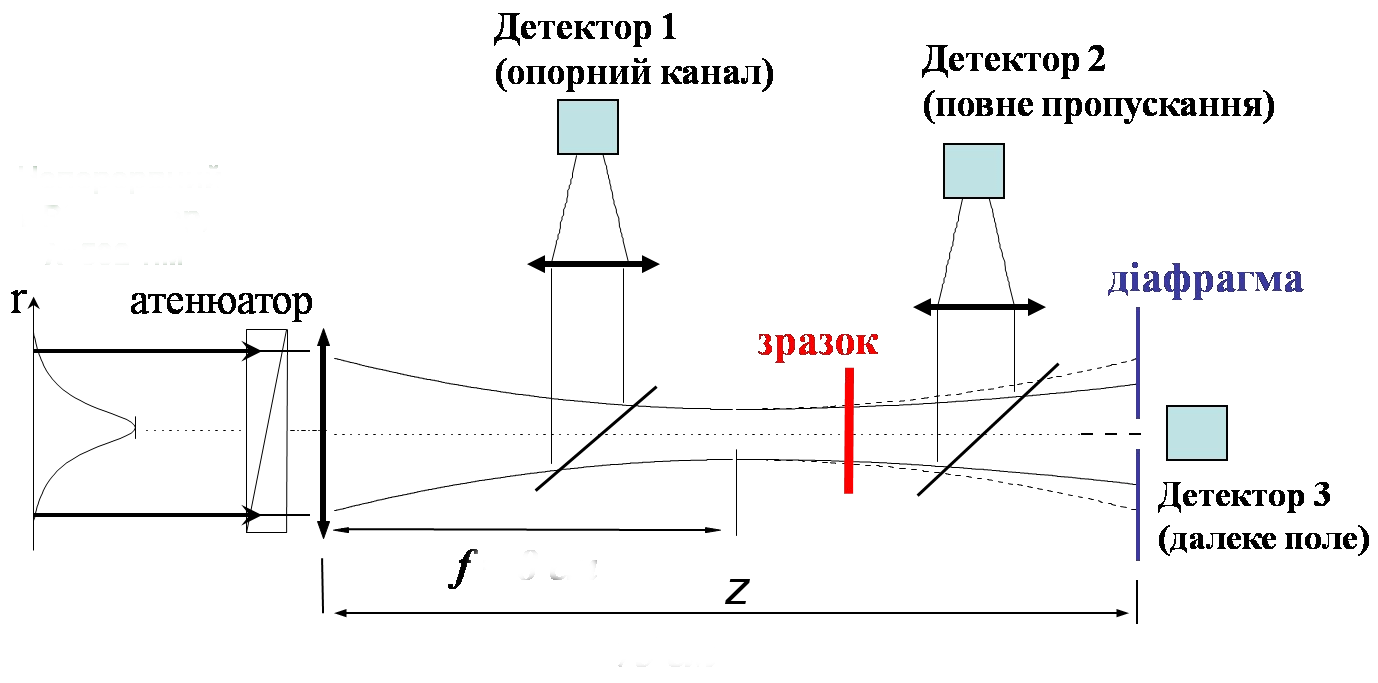
\includegraphics[width=15cm]{s1}
\caption{Оптична схема дослідження фотоіндукованої зміни профілю
пучка в далекому полі. L -- лінза з фокусною відстанню f; П1,П2 -- поділювачі.}\label{fig:s1}
\end{figure}


\section{Теоретичні основи дослідження самовпливу та розрахунку НЛО коефіцієнтів }\label{sec:T_NLO}

При використанні лазерів в якості джерел збудження, за умови великої
інтенсивності випромінювання, зв’язок між поляризацією середовища \textbf{P} і
полем \textbf{E} втрачає лінійний характер (границя застосовності законів лінійної
оптики) і записується як:

\begin{equation}\label{eq:P_main}
P = \chi E + \chi^{(2)} E^2 + \chi^{(3)} E^3 + \dots 
\end{equation}


Коефіцієнти $\chi,~\chi^{(2)},~\chi^{(3)}\dots$ в (\ref{eq:P_main}) залежать від властивостей середовища і називаються оптичними сприйнятливостями. Зокрема, $\chi$ -- лінійна оптична сприйнятливість, $\chi^{(2)}$ -- нелінійна сприйнятливість другого порядку, $\chi^{(3)}$ -- нелінійна сприйнятливість третього порядку і т.д. Нелінійна залежність поляризації середовища від зовнішнього поля призводить до самовпливу лазерного випромінювання, взаємодії лазерних пучків між собою та порушення принципу суперпозиції. 

В ізотропних середовищах або кристалічних структурах з центром інверсії найнижчою нелінійністю, відмінною від нуля, є кубічна нелінійність $\chi^{(3)}$. В наближенні безінерційного відгуку матеріальне рівняння такого середовища має вигляд:

\begin{equation}\label{eq:P}
P=\chi E+ \chi^{(3)}E^3
\end{equation}

Показник заломлення нелінійного середовища можна представити в вигляді:

\begin{equation}
n = n_0 + n_{NLO}(I)
\end{equation}
де $n_0$ -- показник заломлення в лінійному наближенні, $I$ -- інтенсивність світлової хвилі, $n_{NLO}(I)$ -- нелінійна складова, вид якої визначається конкретним механізмом нелінійного відгуку середовища. В найпростішому випадку нелінійну частину
можна представити у вигляді ряду по степеням інтенсивності світлової хвилі:
\begin{equation}\label{eq:n_nlo}
n_{NLO} = n_2 I + n_4 I^2 + \dots
\end{equation}

В більшості експериментів самовплив визначається найнижчим членом
розкладу в \ref{eq:n_nlo} (керрівська нелінійність). Тоді формула для показника заломлення матиме викляд: 

\begin{equation}\label{eq:n_n2}
n_{NLO} = n_2 I + n_4 I^2 + \dots
\end{equation}

Величина $n_2$ , що має розмірність оберненої інтенсивності світла, є зручною характеристикою кубічної нелінійності середовища.

Коефіцієнт оптичного поглинання також має залежність від інтенсивності, яку в найпростішому випадку можна виразити формулою:
\begin{equation}\label{eq:alpha}
\alpha = \alpha_0 + \beta I
\end{equation}
де $\beta$ - коефіцієнт двохфотонного поглинання(ДФП).

По фотоіндукованим змінам повного пропускання можна розрахувати
зміну коефіцієнту поглинання $\Delta\alpha$ та значення дійсної та уявної частини кубічної
нелінійної сприйнятливості $Im(\chi^{(3)})$ за формулою (в одиницях СГС$_e$):
\begin{equation}\label{eq:Im_chi3}
\begin{split}
Im(\chi^{(3)}) &= \frac{{n_0}^2c\lambda}{19.2\pi^3} \cdot \beta \quad\quad \Big[\frac{\text{см}} {\text{МВт}} \Big], \\
Re(\chi^{(3)}) &= 3 \cdot \Big(\frac{n_0}{4\pi}\Big)^2 \cdot n_2 \quad\quad \Big[\frac{\text{см}^2} {\text{кВт}} \Big]
\end{split}
\end{equation}


За законом Бугера-Ламберта-Бера поширення світла в лінійному оптичному середовищі описується можна описати формулою, що в диференційній формі матиме вигляд:
\begin{equation}
dI = -\alpha I dx
\end{equation}

Тут $I$ - інтенсивність світла в об'ємі зразка з товщиною $dx$. При великих
інтенсивностях коефіцієнт поглинання $\alpha$ починає залежати від $I$, причому в
найпростішому випадку ця залежність лінійна. Тоді маємо:

\begin{equation}\label{eq:dI1}
dI = -(\alpha_0 I + \beta I^2 )dx
\end{equation}

Розділення змінних та інтегрування \ref{eq:dI1} дає з урахуванням повної товщини зразка $L$ і падаючої інтенсивності $I_0$ формулу:

\begin{equation}
I(L) = \frac{I_0 e^{-\alpha L}}{ 1 + \beta I_0 L_{eff}}
\end{equation}
де $L_{eff}$ - ефективна довжина середовища, що визначається за формулою:

\begin{equation}\label{eq:L_eff1}
L_{eff} = \frac{1-e^{-\alpha L}}{\alpha}
\end{equation}

Формула \ref{eq:L_eff1} отримана для плоскої хвилі і не описує просторово-часову поведінку пучка. Врахуємо гаусовість просторового розподілу пучка:
\begin{equation}
I = I_0 \exp{(-\frac{r^2}{a^2})}
\end{equation}
 
Коефіцієнт пропускання $T$, який є відношенням повної інтенсивності в пучку, що пройшов крізь зразок, до інтенсивності пучка, що падає, записується в наступному вигляді:


\begin{equation}\label{eq:T1}
T = \frac{\int d \varphi \int r dr \frac{I_0 \exp{(-(\alpha L +\frac{r^2}{a^2}))}}{1+\beta L_{eff} I_0 \exp{(-r^2/a^2)}}}
{\int d\varphi\int r dr I_0 \exp{(-r^2/a^2)}}
\end{equation}

Інтегруючи  \ref{eq:T1} отримаємо:

\begin{equation}\label{eq:T2}
T = \frac{1}{q} \ln{(1+q)} e^{-\alpha L} =\frac{1}{q}\ln{(1+q)}  T_{lin}
\end{equation}

де $q$ визначається з співвідношення:
\begin{equation}\label{eq:q}
q = \beta I_0 L_{eff}
\end{equation}

Модель ДФП є найпростішою для опису нелінійно-оптичних властивостей матеріалу по повному пропусканню, але реально один механізм нелінійності в чистому вигляді практично ніколи не реалізується.
Однак, на різних ділянках реальної кривої залежності $T(I_0)$ можливий розрахунок
ефективних значень $\beta_{eff}$ шляхом апроксимації функцією \ref{eq:T2}.


В наближені тонкого прозорого зразка (коли можна знехтувати НЛО
поглинанням та зміною профілю в товщі зразка внаслідок НЛО
ефектів) амплітуда електричного поля пучка з гаусовим профілем, що пройшов крізь зразок з кубічним НЛО відгуком, може бути записана у вигляді суперпозиції гаусових пучків з різними радіусами пучка та кривизни хвильового фронту. Пучок, що пройшов крізь нелінійно-оптичний зразок з показником заломлення $n(r) = n_0 + n_2 I(r)$ і отримав нелінійний набіг фази $\varphi_{nl} = k n_2 I(r) L_{eff}$, матиме наступну амплітуду:

\begin{equation}\label{eq:E}
E(r) = E_0 \exp{\Bigl(\frac{-\alpha L}{2}\Bigl)} \sum_{m}^{\infty} \frac{[i\varphi_{nl}]^m}{m!} \cdot \frac{w_{m0}}{w_m} \cdot \exp{ \Bigl( - \frac{r^2}{w_{m}^{2}} - \frac{i k r^2}{R_m} + i \theta_m \Bigl)}
\end{equation}

де $E_0$ – амплітуда лазерного поля, що падає на зразок, $r$ – поперечна координата, $w$ і $R$ -- радіус і
кривизна хвильового фронту лазерного променя відповідно, на площині поверхні
зразка; $\alpha$ -- коефіцієнт лінійного поглинання, $d$ -- відстань від зразка до детектора, $w_{m0}$, $w_m$, $R_m$ і $\theta_m$ -- параметри, що
визначаються з геометрії експерименту:


\begin{equation}
\begin{split}
w_{m0}^2 &= \frac{w^2}{2 m +1}\\
d_m &= \frac{k w_{m0}^2}{2}\\
\theta_m &= \tan^{-1} \Big[\frac{d}{d_m \cdot \textit{g}}\Big]
\end{split}
\quad\quad\quad
\begin{split}
 w_m^2 &= w_{m0}^2 [\textit{g}^2 + \Big( \frac{d}{d_m}\Big)^2]\\
 R_m &= d \Big[1-\frac{\textit{g}}{\textit{g}^2 + \Big( \frac{d}{d_.}\Big)^2}\Big]\\
 \textit{g} &= 1 + \frac{d}{R}
\end{split}
\end{equation}

Щоб отримати приосьове пропускання, треба проінтегрувати квадрат модуля амплітуди \ref{eq:E} поля лазера по апертурі діафрагми, а потім нормуванням на потужність пучка. Аналітичний вираз для приосьового пропускання:
\begin{equation}\label{eq:T3}
T ( I_0 ) = S \cdot [1 + a_1 \cdot \varphi_{nl} + a_2 \cdot \varphi_{nl}^2 + a_3 \cdot \varphi_{nl}^3 + \dots] 
\end{equation}

де $S$ і $a_i$ є коефіцієнтами, що визначаються з геометрії експерименту:

\begin{equation}
\begin{split}
S &= 1 - \exp\Big\{ -\frac{ 2( r_0 k w)^2 }{4 z^2 (1 + \beta^2 )} \Big\},\\
a_1 &= \frac{1}{S} \exp{\Big( - \frac{4r_0^2(3+b^2)}{w^2(9+b^2)} \Big)}\sin{\Big(  \frac{8r_0^2 b}{w^2 (9+b^2)}\Big)}\\
a_2 &= \frac{1}{3S}\Big[ \exp{\Big( -\frac{6r_0^2(5+b^2)}{w^2(25+b^2)}\Big)} \cdot \cos{\Big( \frac{24br_0^2}{w^2 (25+b^2)}\Big)}    - \exp{\Big( - \frac{6r_0^2(1+b^2)}{w^2(9+b^2)}\Big)}   \Big]\\
b &= - (1-\frac{z}{R})\Big(\frac{2z}{kw^2}\Big)^{-1}
\end{split}
\end{equation}

Тут $r_0$, -- радіус апертури діафрагми, $b$ -- відношення геоматричної робіжності (результуюча дія оптичної системи) і дифракційної розбіжності лазерного пучка. Параметр $S$ можна розглядати, як пропускання крізь діафрагму Д для системи за відсутності зразка.

Чисельне значення НЛО набігу фази $\varphi_{nl}$ визначається як параметр при
апроксимації експериментальних даних залежностей пропускання крізь діафрагму
від інтенсивності лазерного пучка за моделлю \ref{eq:T3}, де коефіцієнти $a_i$
розраховуються відповідно до умов геометрії експерименту.



%\section{Принцип розрахунку НЛО коефіцієнтів по змінам приосьового пропускання}
%
%
%\section{Принцип розрахунку НЛО коефіцієнтів по фотоіндукованим змінам оптичного пропускання}